\documentclass[12pt, letterpaper]{article}

\usepackage{graphicx}
\usepackage{caption}
\usepackage{amsmath}
\captionsetup[figure]{font=small, labelfont=bf}

\title{Compton Scattering}
\author{Jay Shen}
\date{December 2024}

\begin{document}

\maketitle

\section{Results}

\begin{figure}[!h]
    \centering
    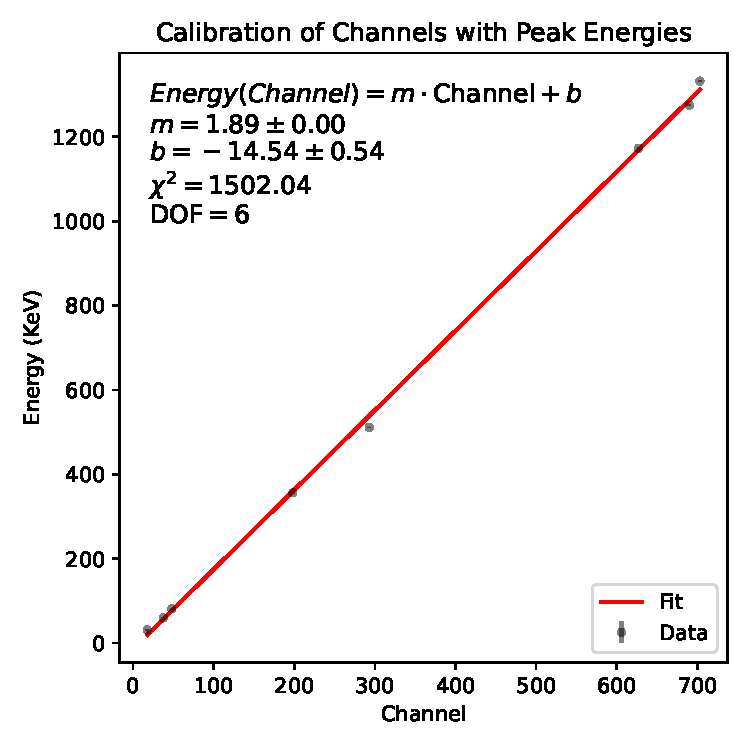
\includegraphics[width=0.5\textwidth]{experiment2/figures/calibration.pdf}
    \caption{}
    \label{fig:cs137-spectrum}
\end{figure}

\begin{table}[h]
\centering
\begin{tabular}{|c | c c c c c c c |}
    \hline
    Energy (KeV) & 31 & 32 & 81 & 356 & 511 & 662 & 1275 \\
    \hline
    Fitted $\lambda$ & 127.9 & 194.7 & 49.7 & 26.8 & 21.3 & 19.1 & 14.7 \\
    Expected $\lambda$ & 279.2 & 256.7 & 54.1 & 26.7 & 22.6 & 20.2 & 14.7 \\
    \hline
\end{tabular}
\caption{Fitted and expected linear attenuation coefficients for various energy levels.}
\label{table:1}
\end{table}

\end{document}